\begin{frame}
    \frametitle{MySQL -Driver JDBC}
    \begin{block}{MySQL}
    	\begin{itemize}
    		\item Système de gestion de bases de données relationnelles
    		\item Libre, gratuit, open-source
    	\end{itemize}
    \end{block}
     \begin{block}{Driver Java DataBase Connectivity }
     	\begin{columns}
  				\begin{column}{5cm}
  					\begin{itemize}
  						\item Connexion/Déconnexion
  						\item Requête : Statement 
  						\item Résultat : ResulSet
  					\end{itemize}
  				\end{column}
  				\begin{column}{5cm}
  				      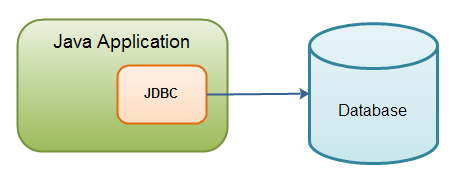
\includegraphics[scale=0.4]{images/jdbc.png}
  				\end{column}
  			\end{columns}

    \end{block}

\end{frame}

\begin{frame}
    \frametitle{Modèle DAO - Principe général}
    \begin{block}{Data Access Object}
    		\begin{itemize}
    			\item Isoler les méthodes concernant le stockage et l'accès aux données
    			\item Création d'une couche supplémentaire :
    		\end{itemize}
    		\center
    		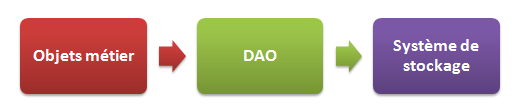
\includegraphics[scale=0.5]{images/dao1.png}
	\end{block}

\end{frame}

\begin{frame}
    \frametitle{Modèle DAO - Mise en place}
     	\begin{columns}
  				\begin{column}{4cm}
  				\begin{block}{Couche DAO}
  				
  					\begin{itemize}
  						\item Méthodes CRUD
  						\item Gestion Exception
  						\item Fabrique 
  						\item Mapping objet-relationnel
  					\end{itemize}
  				\end{block}

  				\end{column}
  				\begin{column}{7cm}
  				      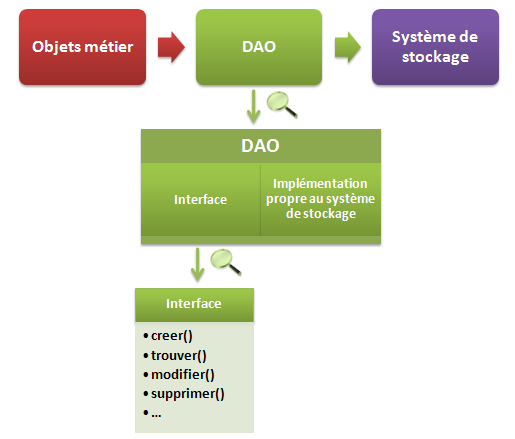
\includegraphics[scale=0.4]{images/dao2.png}
  				\end{column}
  			\end{columns}

\end{frame}